\documentclass[journal,12pt,twocolumn]{IEEEtran}
\usepackage[utf8]{inputenc}
\usepackage{amsmath}
\usepackage{graphicx}
\usepackage[english]{babel}
\usepackage{hyperref}
\usepackage{tcolorbox}
\urlstyle{same}
\title{Assignment  }
\author{Harshal Verma\\
AI21MTECH02003}
\date{April 2021}
\begin{document}
\maketitle
\section{GATE 7}
Problem: Given Set A = [2,3,4,5] and Set B =
[11,12,13,14,15], two numbers are randomly
selected,one from each set. What is probability
that the sum of the two numbers equals 16? \\
(a) 0.20\\
(b) 0.25\\
(c) 0.30\\
(d) 0.33
\\
\\
\\
\\
\textbf{Solution }
Given A = [2,3,4,5] and Set B = [11,12,13,14,15] . the possible combinations of selecting one number from each set is :\\
\\
=  {(2,11),(2,12),(2,13),(2,14),(2,15),(3,11),(3,12),(3,13),\\(3,14),(3,15),(4,11),(,4,12),(4,13),(4,14),(4,15),(5,11),\\(5,12),(5,13),(5,14),(5,15)}\\
\\
From the above sample space have a cardinality of 20 . The samples that sums up to 16 are \\
= {(2,14),(3,13),(4,12),(5,11)}\\
\smallskip
Cardinality of the favourable events is : 4
\smallskip
\begin{align*}
probability &= \frac{\text{favourable sample space}}{\text{Total number of outcomes }}\\
probability &= \frac{4}{20}\\
probability &= 0.2
\end{align*}
\smallskip
The required probability of getting a sum of 16 when choosing two numbers in random is 0.2 \\
\smallskip

\begin{figure}[htp]
    \centering
    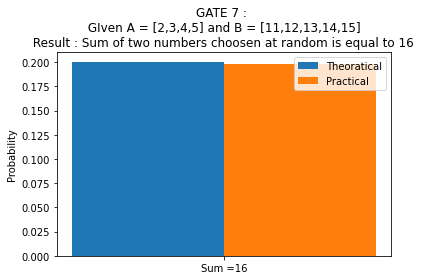
\includegraphics[width=10cm]{Assignemnt_8}
    \label{fig :plot}
\end{figure}

\begin{tcolorbox}
Code source: \url{https://github.com/harshal9876/AI5002/blob/main/Assignment_8/Codes/Assignemnt_8.py} \\
LaTex code :
\url{https://github.com/harshal9876/AI5002/blob/main/Assignment_8/Assignment_8.tex}
\end{tcolorbox}
\vfill
\end{document}




